% Diese Datei ist Teil des Buchs "Schreibe Dein Programm!"
% Das Buch ist lizensiert unter der Creative-Commons-Lizenz
% "Namensnennung - Weitergabe unter gleichen Bedingungen 4.0 International (CC BY-SA 4.0)"
% https://creativecommons.org/licenses/by-sa/4.0/deed.de

\chapter{Programmieren mit Akkumulatoren}
\label{cha:accu}

Manche Berechnungen funktionieren am einfachsten, wenn sie ein
Zwischenergebnis mitführen und aktualisieren.  Die bisherigen
Konstruktionsanleitungen für Funktionen, die Listen oder natürliche
Zahlen verarbeiten, können das aber nicht.  Wir brauchen dafür eine
neue Programmiertechnik, das Programmieren mit
\textit{Akkumulatoren}, und entsprechend angepasste
Konstruktionsanleitungen.  Beides behandeln wir in diesem Kapitel.

\section{Zwischenergebnisse mitführen}
\label{sec:intermediate-results}

\mentioncode{akkumulatoren/accumulator.rkt}
%
Wir fangen mit einer scheinbar einfachen Funktion an: Gefragt ist eine
Funktion, die eine Liste invertiert, also die Reihenfolge ihrer
Elemente umdreht:\indexvariable{invert}\label{sec:invert}
%
\begin{lstlisting}
; Liste umdrehen
(: invert ((list-of %a) -> (list-of %a)))

(check-expect (invert empty) empty)
(check-expect (invert (list 1 2 3 4)) (list 4 3 2 1))
\end{lstlisting}
%
Gerüst und Schablone sehen wie folgt aus:
%
\begin{lstlisting}
(define invert
  (lambda (list)
    (cond
      ((empty? list) ...)
      ((cons? list)
      ... (invert (rest list)) ...
      ... (first list) ...))))
\end{lstlisting}
%
Um den Rumpf zu vervollständigen, können wir uns an dem zweiten
Testfall orientieren~-- da ist \lstinline{list} die Liste mit den
Elementen 1 2 3 4.  Entsprechend ist \lstinline{(first list)} die
Zahl 1, \lstinline{(rest list)} die Liste mit den Elementen 2 3 4, das
heiß der rekursive Aufruf liefert die Liste mit den Elementen 4 3 2.
Um das gewünschte Ergebnis mit den Elementen 4 3 2 1 zu bekommen,
müssen wir deshalb \lstinline{(first list)} hinten an das Ergebnis des
rekursiven Aufrufs anhängen.

Um ein Element \emph{hinten} an eine Liste zu hängen, haben wir bisher
noch keine fertige Funktion~-- die müssen wir erst noch schreiben.
Wir könnten die Arbeit jetzt unterbrechen, um das zu tun.  Wir machen
erstmal nur eine Notiz, dass wir das später machen~-- in Form einer
Kurzbeschreibung und einer Signatur:
%
\begin{lstlisting}
; Element an Liste anhängen
(: append-element ((list-of %a) %a -> (list-of %a)))
\end{lstlisting}
%
Wenn wir diese Funktion voraussetzen, können wir \lstinline{invert}
recht einfach fertigschreiben:
%
\indexvariable{invert}
\begin{lstlisting}
(define invert
  (lambda (list)
    (cond
      ((empty? list) empty)
      ((cons? list)
       (append-element (invert (rest list))
                       (first list))))))
\end{lstlisting}
%
Die Funktion \lstinline{append-element} ist ganz ähnlich der Funktion
\lstinline{concatenate} aus Abschnitt~\ref{sec:more-lists}.  Zunächst
Testfälle:
%
\begin{lstlisting}
(check-expect (append-element (list 1 2 3) 4) (list 1 2 3 4))
(check-expect (append-element empty 4) (list 4))
\end{lstlisting}
%
Gerüst und Schablone:
%
\begin{lstlisting}
(define append-element
  (lambda (list element)
    (cond
      ((empty? list) ...)
      ((cons? list)
       ... (first list) ...
       ... (append-element (rest list) element) ...))))
\end{lstlisting}
%
Im \lstinline{cons}-Fall können wir auch hier die Lösung anhand eines
Beispiels finden: Im Testfall hat \lstinline{list} die Elemente 1 2 3,
der rekursive Aufruf liefert also 2 3 4.  Wir müssen
\lstinline{(first list)}, also die 1, nur noch vorne dranhängen, mit
\lstinline{cons}. Im \lstinline{empty}-Fall hängen wir
\lstinline{element} hinten an eine leere Liste~-- wir brauchen deshalb
eine einelementige Liste mit \lstinline{element} drin, das könnten wir
mit der eingebauten \lstinline{list} machen:
%
\begin{lstlisting}
(define append-element
  (lambda (list element)
    (cond
      ((empty? list) (list element))
      ((cons? list)
       (cons (first list)
             (append-element (rest list) element))))))
\end{lstlisting}
%
Hier wollten wir gern "<Fertig!"> wie sonst auch schreiben, aber die
Funktion funktioniert nicht: DrRacket beschwert sich, dass nach der
öffnenden Klammer von \lstinline{(list element)} keine Funktion steht
sondern \lstinline{#<empty-list>}.  Wups!  Das liegt daran, dass wir
zwar in \lstinline{(list element)} die eingebaute Funktion
\lstinline{list} gemeint haben,
wir aber auch einen Parameter mit dem Namen \lstinline{list}
benutzen, und der
überdeckt nach den Regeln der lexikalischen Bindung aus
Abschnitt~\ref{sec:lexikalische-bindung} auf
Seite~\pageref{sec:lexikalische-bindung} die
eingebaute Funktion.

Wir können das Problem auf zwei Arten lösen~-- wir benennen den
Parameter um oder wir konstruieren die einelementige Liste "<von
Hand">.  Wir haben uns für letzteres entschieden:
%
\indexvariable{append-element}
\begin{lstlisting}
(define append-element
  (lambda (list element)
    (cond
      ((empty? list) (cons element empty))
      ((cons? list)
       (cons (first list)
             (append-element (rest list) element))))))
\end{lstlisting}

Doch zurück zu \lstinline{invert}.  Schon das Invertieren von Listen der Länge
1000 eine ganze Weile.  Du kannst das ausprobieren, indem
Du die Funktion \lstinline{copies} aus Abschnitt~\ref{func:copies} auf
Seite~\pageref{func:copies} verwendest und das hier in der REPL auswertest:
%
\begin{lstlisting}
(invert (copies 1000 42))
\end{lstlisting}
%
Das dauert auf dem alten Computer von Michael
Sperber immerhin ein
paar Sekunden: Das wäre vielleicht in den 70er Jahren noch akzeptabel
gewesen.  
Das Invertieren einer Liste der Länge 400 dauert \emph{mehr} als doppelt so
lang wie das Invertieren einer Liste der Länge 200 benötigt.  Das
liegt daran, dass \lstinline{invert} bei jedem rekursiven Aufruf
\lstinline{append-element} aufruft, und \lstinline{append-element} selbst
macht soviele rekursive Aufrufe wie die Liste lang ist. Das sind für
eine Liste der Länge 20 für den ersten Aufruf von
\lstinline{append-element} 19 Aufrufe, für den zweiten 18 Aufrufe
undsoweiter.

Das sind also $19+18+17+\ldots+1$ rekursive Aufrufe.  Vielleicht
erinnerst Du Dich~-- das ist ein Beispiel für die Gaußsche
Summenformel, siehe Abschnitt~\ref{sec:gausssche-summenformel}
auf Seite~\pageref{sec:gausssche-summenformel}:
%
\[\forall n\in\mathbb{N}: \sum_{i=0}^n i =
  \frac{n\times (n+1)}{2}\]
%
\begin{figure}[tb]
  \centering
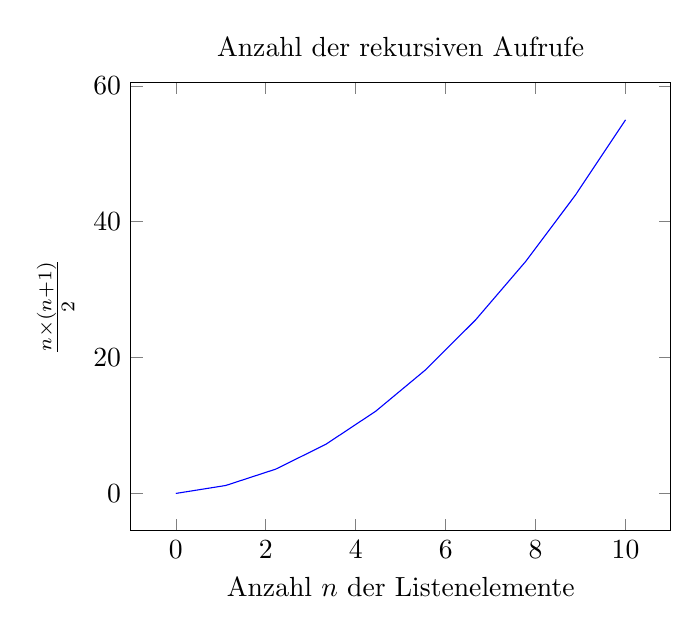
\begin{tikzpicture}
  \begin{axis}[
    title={Anzahl der rekursiven Aufrufe},
    xlabel={Anzahl $n$ der Listenelemente},
    ylabel={$\frac{n\times (n+1)}{2}$}
    ]
    \addplot [
    blue,
    domain=0:10,
    samples=10,
    ]
    {x*(x+1)/2};
  \end{axis}
\end{tikzpicture}
  \caption{Funktionaufrufe bei \lstinline{invert}}
  \label{fig:invert-calls}
\end{figure}

\noindent Wenn Du diese Formel für immer größer werdende $n$ ausrechnest, wird
die Zahl schwindelerregend schnell größer, wie
Abbildung~\ref{fig:invert-calls} zeigt.  Woran liegt das?

Wenn Du die rechte Seite ausmultiplizierst, steht da:
\[ \frac{n\times (n+1)}{2} = \frac{n^2 + n}{2} \]
%
In der Formel bestimmt das $n^2$ das schnelle Wachstum, auch
\textit{quadratisch} genannt.\index{quadratisches Wachstum}

Zum Glück gibt es eine bessere Methode, eine Liste umzudrehen: Die
obige \lstinline{invert}"=Funktion konstruiert die Ergebnisliste, indem
stets Elemente \emph{hinten} angehängt werden.  Das entspricht 
nicht der "<natürlichen"> Konstruktion von Listen mit
\lstinline{cons}, das ein Element \emph{vorn} anhängt.  
Das Ergebnis ließe sich durch Anhängen vorn ganz einfach
konstruieren, indem in folgender Reihenfolge
Zwischenergebnisse\index{Zwischenergebnis} berechnet werden, wie hier für den
Testfall \lstinline{(invert (list 1 2 3 4))}:
%
\begin{lstlisting}
#<empty-list>
#<list 1>
#<list 2 1>
#<list 3 2 1>
#<list 4 3 2 1>
\end{lstlisting}
%
Jedes Zwischenergebnis entsteht aus dem vorhergehenden, indem ein
Element vorn an die Liste darüber angehängt wird.  Dies geschieht in
der Reihenfolge, in der die Elemente in der ursprünglichen Liste
auftreten: scheinbar einfach.  Allerdings erlaubt die normale
Konstruktionsanleitung für Listen nicht, dieses Zwischenergebnis
mitzuführen: Das Ergebnis des rekursiven Aufrufs
\lstinline{(invert (rest lis))} ist unabhängig vom Wert von
\lstinline{(first lis)}.  Damit aber
ist es der Funktion aus der normalen Konstruktionsanleitung unmöglich,
die obige Folge von Zwischenergebnissen nachzuvollziehen, da von einem
Zwischenergebnis zum nächsten gerade \lstinline{(first lis)} vorn
angehängt wird.  Wir müssen also etwas anders an das Problem herangehen.

Um das Zwischenergebnis mitzuführen, 
benutzen wir einen separaten Parameter, einen sogenannten
\textit{Akkumulator\index{Akkumulator}}.  Dieser sammelt die
invertierte Liste der bisher schon "<gesehenen"> Elemente auf.  Hier
ist die Signatur der neuen Funktion \lstinline{invert-helper}:
%
\begin{lstlisting}
; Hilfsfunktion zum Umdrehen einer Liste
(: invert-helper ((list-of %a) (list-of %a) -> (list-of %a)))
\end{lstlisting}
%
Der folgende Testfall soll illustrieren, wie die Funktion arbeitet:
\begin{lstlisting}
(check-expect (invert-helper (list 4 5 6) (list 3 2 1))
              (list 6 5 4 3 2 1))
\end{lstlisting}
%
Die zweite Liste~-- der Akkumulator~-- enthält die "<bereits
invertierten"> Elemente.  Die erste Liste ist noch nicht verarbeitet;
die Elemente werden nacheinander an den Akkumulator vorn drangehängt.
Für die Definition der Funktion setzen wir erst einmal die bereits
bekannte Schablone ein für Funktionen, die eine Liste akzeptieren:
%
\begin{lstlisting}
(define invert-helper
  (lambda (list inverted)
    (cond
      ((empty? list) ...)
      ((cons? list)
       ... (first list) ...
       ... (invert-helper (rest list) ...) ...))))
\end{lstlisting}
%
Ziemlich viele Lücken noch!  Füllen wir erstmal die einfachste, im
\lstinline{empty}-Fall: Dann nämlich hat die Funktion schon "<alle
Elemente gesehen"> und diese in den Akkumulator \lstinline{inverted}
"<hineinakkumuliert">~-- der enthält dann die invertierte
Eingabeliste:
%
\begin{lstlisting}
(define invert-helper
  (lambda (list inverted)
    (cond
      ((empty? list) inverted)
      ((cons? list)
       ... (first list) ...
       ... (invert-helper (rest list) ...) ...))))
\end{lstlisting}
%
Im \lstinline{cons}-Fall müssen wir das Argument zum zweiten
Parameter von \lstinline{invert-helper} ergänzen: Wir sind natürlich
versucht, da einfach \lstinline{inverted} hinzuschreiben wie bei
vielen anderen rekursiven Funktionen vorher.  Aber wir müssen doch die
Elemente von \lstinline{list} da noch "<hineinakkumulieren"> und aus
dem vorigen Zwischenergebnis das nächste machen.  Für das
"<Hineinakkumulieren"> nehmen wir das erste Element und hängen es
vorn an, so wie wir es in der Beispielrechnung auch gemacht haben:
%
\begin{lstlisting}
(define invert-helper
  (lambda (list inverted)
    (cond
      ((empty? list) inverted)
      ((cons? list)
       ...
       (invert-helper (rest list)
                      (cons (first list) inverted))
       ...))))
\end{lstlisting}
%
Was müssen wir noch dazuschreiben?  Die Funktion arbeitet schon die
Eingabeliste ab und akkumuliert ihre Elemente in \lstinline{inverted}
hinein. Sie ist bereits fertig, wir müssen nur die Ellipsen wegmachen:\label{function:invert-helper}
%
\indexvariable{invert-helper}
\begin{lstlisting}
(define invert-helper
  (lambda (list inverted)
    (cond
      ((empty? list) inverted)
      ((cons? list)
       (invert-helper (rest list)
                      (cons (first list) inverted))))))
\end{lstlisting}
%
Die Funktion kann schon was, ist aber nicht identisch zur
ursprünglichen \lstinline{invert}-Funktion, die ja nur eine Eingabe
hat.  Um "<einfach nur eine Liste umzudrehen">, können wir
\lstinline{invert-helper} mit einem leeren Akkumulator aufrufen, wie
in diesem Testfall:
%
\begin{lstlisting}
(check-expect (invert-helper (list 1 2 3) empty)
              (list 3 2 1))
\end{lstlisting}
%
\begin{aufgabeinline}
  Definiere \lstinline{invert} um, so dass es
  \lstinline{invert-helper} benutzt!
\end{aufgabeinline}
%
Die neue Version von \lstinline{invert} benutzt keine Hilfsfunktion und
macht soviele rekursive Aufrufe wie die Eingabeliste Elemente hat, ihre
Laufzeit wächst also \textit{linear}.\index{lineares Wachstum}

Die Funktion \lstinline{invert} ist so nützlich,
dass sie unter dem Namen
\lstinline{reverse}\indexvariable{reverse} eingebaut ist.

\section{Schablonen für Funktionen mit Akkumulator}

Auch für Funktionen mit Akkumulator entwickeln wir eine
Konstruktionsanleitung.  Vorher wollen wir aber noch einmal
anhand eines weiteren Beispiels Revue passieren lassen, wie der
Konstruktionsprozess bei solchen Funktionen eigentlich genau aussieht.
Wir nehmen uns eine Funktion vor, die wir eigentlich schon kennen,
nämlich aus Abschnitt~\ref{sec:list-sum} auf Seite
\pageref{sec:list-sum}:\label{function:list-sum-acc}
%
\begin{lstlisting}
; Summe der Elemente einer Liste von Zahlen berechnen
(: list-sum ((list-of number) -> number))
\end{lstlisting}
%
Wir nehmen uns allerdings diesmal vor, mit Akkumulator zu arbeiten.
Dazu müssen wir uns überlegen, was für Information der
Akkumulator eigentlich akkumulieren soll.  Das sollte ein
\textit{Zwischenergebnis}\index{Zwischenergebnis} sein, 
eine vorläufige Version des gewünschten Endergebnisses.  Da 
hier das Endergebnis die Summe aller Listenelemente ist, nehmen wir
als Zwischenergebnis die Summe aller Listenelemente, die unsere
Funktion schon "<gesehen"> hat und nennen es \lstinline{sum}.  Wir schreiben folgende Schablone:
%
\indexvariable{list-sum-helper}
\begin{lstlisting}
(define list-sum-helper
  (lambda (list sum)
    (cond
      ((empty? list) ... sum ...)
      ((cons? list)
       (list-sum-helper (rest list)
                        (... (first list) ... sum ...))))))
\end{lstlisting}
%
Warum sieht sie gerade so aus, beziehungsweise: Was ist der Unterschied
zur ganz normalen Schablone für Listen als Eingabe aus
Konstruktionsanleitung~\ref{ka:listen-eingabe-schablone} auf
Seite~\pageref{ka:listen-eingabe-schablone}?   Hier ist sie zur
Erinnerung noch einmal:
%
\begin{lstlisting}
(define |\(f\)|
  (lambda (|\ldots| |\(\mathit{list}\)| |\ldots|)
    (cond
      ((empty? |\(\mathit{list}\)|) |\ldots|)
      ((cons? |\(\mathit{list}\)|)
       |\ldots|
       (first |\(\mathit{list}\)|)
       (|\(f\)| (first |\(\mathit{list}\)|))
       |\ldots|
       ))))
\end{lstlisting}
%
Im \lstinline{empty}-Zweig steht der Akkumulator \lstinline{sum},
während in
der Schablone aus
Konstruktionsanleitung~\ref{ka:listen-eingabe-schablone} gar nichts
steht: Hier ist die Liste am Ende und es ist Zeit, das Endergebnis
auszurechnen, das im \lstinline{empty}-Zweig herauskommen soll.   Weil
der Akkumulator ein Zwischenergebnis ist, muss er am Schluss zumindest
nah am
Endergebnis dran sein.  Meist \emph{ist} das letzte
Zwischenergebnis das Endergebnis.

Im \lstinline{cons}-Fall steht ein rekursiver Aufruf mit
\lstinline{(rest list)} als Listen-Argument~-- wie in
Konstruktionsanleitung~\ref{ka:listen-eingabe-schablone} auch.
Außerdem steht dort eine Hilfestellung für die Berechnung des
Akkumulator"=Arguments, also des nächsten Zwischenergebnisses.  Da
sollte das letzte Zwischenergebnis~-- hier \lstinline{sum}~-- und das
nächste Listenelement \lstinline{(first list)} eingehen. Darum stehen
sie in der Schablone.  Dieser Teil der Schablone ist also nur eine
Erweiterung der ursprünglichen Schablone.

Außerdem fällt Dir vielleicht auf, dass um den rekursiven Aufruf herum
keine Ellipsen \lstinline{...} stehen: Du solltest da nichts drumherum
schreiben.  Das liegt daran, dass der letzte rekursive Aufruf von
\lstinline{list-sum-helper} am Ende der Liste das Ergebnis
produziert~-- das muss die Funktion einfach unverändert zurückliefern,
und darum steht da nichts drumherum.

Um die Funktion zu vervollständigen, müssen wir noch klarer als bisher
formulieren, was genau der Akkumulator \lstinline{sum} repräsentiert.
Oben haben wir etwas salopp geschrieben, dass es sich um die Summe
aller Listenelemente handelt, welche die Funktion schon "<gesehen">
hat.  Die sind aber für \lstinline{list-sum-helper} gar nicht mehr
sichtbar.  Wir können sie sichtbar machen, indem wir die Funktion
\lstinline{list-sum} einbeziehen, die \lstinline{list-sum-helper}
aufruft.  Hier ist die Schablone dafür:
%
\begin{lstlisting}
(define list-sum
  (lambda (list0)
    (list-sum-helper list0 ...)))
\end{lstlisting}
%
Wir haben bewusst den Namen \lstinline{list0} gewählt, damit wir ihn
nicht mit dem \lstinline{list} aus der Funktion \lstinline{list-sum-helper}
durcheinanderbringen.  (Anders als noch bei \lstinline{reverse}~-- wir
versuchen, es besser zu machen.)

\begin{figure}[tb]
  \centering
  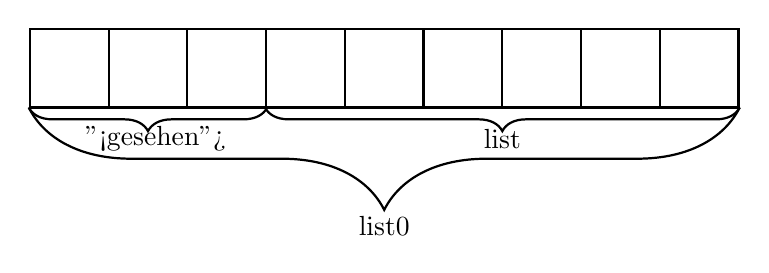
\begin{tikzpicture}
    \node (cell1) at (0,0) [draw,thick,minimum width=1cm,minimum height=1cm] {};
    \node (cell2) at (1,0) [draw,thick,minimum width=1cm,minimum height=1cm] {};
    \node (cell3) at (2,0) [draw,thick,minimum width=1cm,minimum height=1cm] {};
    \node (cell4) at (3,0) [draw,thick,minimum width=1cm,minimum height=1cm] {};
    \node (cell5) at (4,0) [draw,thick,minimum width=1cm,minimum height=1cm] {};
    \node (cell6) at (5,0) [draw,thick,minimum width=1cm,minimum height=1cm] {};
    \node (cell7) at (6,0) [draw,thick,minimum width=1cm,minimum height=1cm] {};
    \node (cell8) at (7,0) [draw,thick,minimum width=1cm,minimum height=1cm] {};
    \node (cell9) at (8,0) [draw,thick,minimum width=1cm,minimum height=1cm] {};
    \draw [
    thick,
    decoration={
        brace,
        amplitude=0.3cm,
        mirror,
        raise=0.5cm
    },
    decorate
    ] (cell4.west) -- (cell9.east) 
    node [midway,yshift=-0.9cm] {\lstinline{list}};
    \draw [
    thick,
    decoration={
        brace,
        amplitude=1.3cm,
        mirror,
        raise=0.5cm
    },
    decorate
    ] (cell1.west) -- (cell9.east) 
    node [midway,yshift=-2cm] {\lstinline{list0}};

    \draw [
    thick,
    decoration={
        brace,
        amplitude=0.3cm,
        mirror,
        raise=0.5cm
    },
    decorate
    ] (cell1.west) -- (cell3.east) 
    node [midway,xshift=0.1cm,yshift=-0.9cm] {"<gesehen">};
  \end{tikzpicture}
  
  \caption{Gesehene Elemente einer Liste in einer Funktion mit Akkumulator}
  \label{fig:list0-list}
\end{figure}

Abbildung~\ref{fig:list0-list} zeigt die Beziehung zwischen
\lstinline{list0} und \lstinline{list}: \lstinline{list0} ist die
Liste \emph{aller} Elemente, \lstinline{list} markiert die Stelle, an
der sich \lstinline{list-sum-helper} gerade befindet, besteht also aus
noch nicht gesehenen Elementen.

Bevor wir nun die Schablone ausfüllen, sollten wir überlegen, in welchem Verhältnis
\lstinline{list0}, \lstinline{list} und \lstinline{sum} stehen.  Hier
ist das nämlich noch einfach, aber bei machen Funktionen mit
Akkumulator werden wir sehen, dass es schwieriger ist.  In diesem Fall
könnte das so aussehen:
%
\begin{center}
  \lstinline{sum} ist die Summer aller Elemente in \lstinline{list0} vor
  \lstinline{list}.
\end{center}
%
Diese Aussage sollten wir als Kommentar in die Funktion schreiben,
denn daraus ergibt sich alles weitere.  Weil sie so wichtig ist, hat
sie einen eigenen Namen: \textit{Invariante}\index{Invariante}.
("<Vario"> heißt im Lateinischen "<sich ändern">, entsprechend
ist eine In-variante etwas, was sich nicht verändert.)

Um die Funktion fertigzustellen, fangen wir damit an, die Lücke in
\lstinline{list-sum} zu schließen, die \lstinline{list-sum-helper} mit
\lstinline{list0} aufruf.  \lstinline{List0} und \lstinline{list} sind
also gleich~-- es gibt keine Elemente "<vor \lstinline{list}">.  Die
Summe dieser leeren Liste ist $0$ und damit auch das Argument im Aufruf
von \lstinline{list-sum-helper}:
%
\indexvariable{list-sum}
\begin{lstlisting}
(define list-sum
  (lambda (list0)
    (list-sum-helper list0 0)))
\end{lstlisting}
%
Als nächstes ist der \lstinline{empty}-Zweig dran.  Hier ist
\lstinline{sum} die Summe aller Elemente vor \lstinline{list}, und,
weil \lstinline{list} leer ist, sind das \emph{alle} Elemente von
\lstinline{list0}.  Deswegen ist \lstinline{sum} das gewünschte
Endergebnis.  Zwischenstand:
%
\begin{lstlisting}
(define list-sum-helper
  ; sum ist die Summe aller Elemente in list0 vor list
  (lambda (list sum)
    (cond
      ((empty? list) sum)
      ((cons? list)
       (list-sum-helper (rest list)
                        (... (first list) ... sum ...))))))
\end{lstlisting}
%
Es bleibt der rekursive Aufruf.  Hier muss der \emph{neue} Wert von
\lstinline{sum} berechnet werden, also die Summe aller Elemente vor
\lstinline{(rest list)}.  Dazu müssen wir auf die bisherige Summe
\lstinline{(first list)} addieren:
%
\indexvariable{list-sum-helper}
\begin{lstlisting}
(define list-sum-helper
  ; sum ist die Summe aller Elemente in list0 vor list
  (lambda (list sum)
    (cond
      ((empty? list) sum)
      ((cons? list)
       (list-sum-helper (rest list) (+ (first list) sum))))))
\end{lstlisting}
%
Fertig!

Also na ja~-- es nervt etwas, immer zwei Funktionen schreiben zu müssen
und immer \lstinline{-helper} dranzuhängen.  Wir können die Funktion
übersichtlicher machen, indem wir \lstinline{list-sum-helper} zu einer
lokalen Definition innerhalb von \lstinline{list-sum} machen:
%
\indexvariable{list-sum}
\begin{lstlisting}
(define list-sum
  (lambda (list0)
    (define list-sum-helper
      ; sum ist die Summer aller Elemente in list0 vor list
      (lambda (list sum)
        (cond
          ((empty? list) sum)
          ((cons? list)
           (list-sum-helper (rest list) (+ (first list) sum))))))
    (list-sum-helper list0 0)))
\end{lstlisting}
%
Außerdem kannst Du, wenn Dich das \lstinline{helper} nervt, einen
knackigeren Namen wählen, der Dir besser gefällt.  Wir nehmen
\lstinline{accumulate}:
%
\begin{lstlisting}
(define list-sum
  (lambda (list0)
    (define accumulate
      ; sum ist die Summer aller Elemente in list0 vor list
      (lambda (list sum)
        (cond
          ((empty? list) sum)
          ((cons? list)
           (accumulate (rest list) (+ (first list) sum))))))
    (accumulate list0 0)))
\end{lstlisting}
%
Aus diesem Beispiel ergibt sich folgende Konstruktionsanleitung:
%
\begin{konstruktionsanleitung}{Listen als Eingabe, mit Akkumulator: Schablone}
  \label{ka:listen-eingabe-akkumulator-schablone}
  Wenn Du eine Funktion schreibst, die eine Liste akzeptiert und
  einen Akkumulator benutzen soll, gehe folgendermaßen vor:
  \begin{enumerate}
  \item Überlege Dir, was für Information der Akkumulator
    repräsentieren soll. Das ist typischerweise ein
    Zwischenergebnis~-- also ein vorläufiger Wert für das
    Endergebnis.  Insbesondere ist die Signatur des Akkumulators die
    gleiche wie die des Endergebnisses.
  \item Konstruiere die Schablone wie folgt:
\begin{lstlisting}
(define |\(f\)|
  (lambda (... |\(\mathit{list}\sb{0}\)| ...)
    (define accumulate
      (lambda (|\(\mathit{list}\)| |\(\mathit{acc}\)|)
        (cond
          ((empty? |\(\mathit{list}\)|) |\ldots| |\(\mathit{acc}\)| |\ldots|)
          ((cons? |\(\mathit{list}\)|)
           (accumulate (rest |\(\mathit{list}\)|) 
                       (... (first |\(\mathit{list}\)|) ... |\(\mathit{acc}\)| ...))))))
    (accumulate |\(\mathit{list}\sb{0}\)| ...)))
\end{lstlisting}
    \item Formuliere eine möglichst konkrete Invariante zwischen
      $\mathit{list}_0$, $\mathit{list}$ und $\mathit{acc}$ und
      schreibe sie als Kommentar zu \lstinline{accumulate}.
    \item Fülle mit Hilfe der Invariante die Ellipsen in der Funktion aus.
  \end{enumerate}
\end{konstruktionsanleitung}
%
Die Konstruktionsanleitung zeigt auch, warum es schwieriger ist, eine
Funktion mit Akkumulator zu schreiben, als eine "<normale"> Funktion,
die Listen akzeptiert: Du musst eine Invariante finden, und dafür gibt
es nur wenig allgemeingültige Hilfestellung.

\begin{aufgabeinline}\label{aufgabe:list-min-nonemepty-acc}
  Schreibe die Funktion \lstinline{list-min-nonempty} aus
  Abschnitt~\ref{sec:list-min-nonempty} auf
  Seite~\pageref{sec:list-min-nonempty} noch einmal, diesmal mit
  Akkumulator.

  Überlege Dir, was der Akkumulator repräsentieren sollte sowie eine
  sinnvolle Invariante!

  Genau wie bei \lstinline{list-min-nonempty} musst Du dafür die
  Konstruktionsanleitung etwas variieren: Die nichtleere Liste kannst
  Du schon vorab in erstes Element und Rest aufteilen und daraus die
  richtigen Eingaben für \lstinline{accumulate} berechnen.
  \lstinline{Accumulate} ist aber wie in der Schablone.
\end{aufgabeinline}
%

\section{Über natürliche Zahlen akkumulieren}

Auch über natürliche Zahlen können wir Funktionen schreiben, die einen
Akkumulator sinnvoll benutzen.  Wir zeigen das anhand der
\lstinline{power}-Funktion, die wir schonmal "<normal"> in
Abschnitt~\ref{function:power} auf Seite~\pageref{function:power}
programmiert haben.

Kurzbeschreibung, Signatur und Tests sind wie gehabt:
%
\begin{lstlisting}
; Potenz einer Zahl berechnen
(: power (number natural -> number))

(check-expect (power 5 0) 1)
(check-expect (power 5 3) 125)
\end{lstlisting}
%
Wir benutzen nun schon von vornherein die gleiche Namenskonvention wie
in
Konstruktionsanleitung~\ref{ka:listen-eingabe-akkumulator-schablone}
und benennen den entscheidenen Parameter mit einer \lstinline{0} am
Ende.
%
\begin{lstlisting}
(define power
  (lambda (base exponent0)
    ...))
\end{lstlisting}
%
Die Schablone entsteht jetzt ganz ähnlich wie bei den Listen: Wir
schreiben eine \lstinline{accumulate}-Funktion mit Parametern
\lstinline{exponent} und \lstinline{acc}.  \lstinline{Accumulate}
macht genau wie in der Schablone aus
Konstruktionsanleitung~\ref{ka:nats-eingabe-schablone} auf
Seite~\pageref{ka:nats-eingabe-schablone} eine Verzweigung nach den
zwei Fällen natürlicher Zahlen.  Der rekursive Aufruf im
\lstinline{positive?}-Zweig muss genau wie dort \lstinline{(- exponent 1)}
übergeben:
%
\begin{lstlisting}
(define power
  (lambda (base exponent0)
    (define accumulate
      (lambda (exponent acc)
        (cond
          ((zero? exponent)
           ... acc ...)
          ((positive? exponent)
           (accumulate (- exponent 1) ... acc ...)))))
    (accumulate exponent0 ...)))
\end{lstlisting}
%
Jetzt müssen wir uns noch überlegen, was \lstinline{acc} eigentlich
sein soll.  Da die Potenz ein wiederholtes Produkt von \lstinline{base}
ist, sollte \lstinline{acc} auch ein Produkt sein.
Während \lstinline{accumulate} jedesmal \lstinline{exponent} um eins
herunterzählt, könnten wir den Akkumulator bei jeder Runde ein
weiteres Mal mit \lstinline{base} multiplizieren~-- ähnlich, wie wir
es vielleicht auch auf einem Zettel machen würden.  Der Akkumulator
ist also eine "<Zwischenpotenz"> und wir nennen ihn deshalb einfach
\lstinline{power}.

Wir sollten noch eine Invariante formulieren, damit auch alles richtig
läuft.  Dafür müssen wir klären, \emph{welche} Zwischenpotenz
\lstinline{power} eigentlich ist.  Da \lstinline{exponent} immer
kleiner wird, bietet sich die Differenz zwischen \lstinline{exponent0}
und \lstinline{exponent} an~-- die fängt bei $0$ an und wird immer
größer.  Das Hütchen \lstinline{^} im Kommentar heißt hier "<hoch">:
%
\begin{lstlisting}
(define power
  (lambda (base exponent0)
    (define accumulate
      ; power ist base^(exponent0 - exponent)
      (lambda (exponent power)
        (cond
          ((zero? exponent) ...)
          ((positive? exponent)
           (accumulate (- exponent 1) ...)))))
    (accumulate exponent0 ...)))
\end{lstlisting}
%
Mit der Invariante können wir die Lücken füllen: Im ersten Zweig
ist \lstinline{exponent} $0$.  Das bedeutet, dass \lstinline{power}
gerade "<\lstinline{base} hoch \lstinline{exponent0}"> ist~-- das
Endergebnis.  Im zweiten Zweig müssen wir entsprechend dem
reduzierten \lstinline{exponent} einmal \lstinline{base} an das
Zwischenergebnis dranmultiplizieren.  Es fehlt nur noch der Wert
für \lstinline{power} im ersten Aufruf von \lstinline{accumulate}.  Da
$b^0 = 1$ ist, müssen wir $1$ einsetzen:
%
\indexvariable{power}
\begin{lstlisting}
(define power
  (lambda (base exponent0)
    (define accumulate
      ; power ist base^(exponent0 - exponent)
      (lambda (exponent power)
        (cond
          ((zero? exponent) power)
          ((positive? exponent)
           (accumulate (- exponent 1) (* power base))))))
    (accumulate exponent0 1)))
\end{lstlisting}
%
Fertig!

Auch für solche Funktionen mit Akkumulator, die natürliche Zahlen
konsumieren, können wir eine Schablone formulieren:

\begin{konstruktionsanleitung}{Natürliche Zahlen als Eingabe, mit Akkumulator: Schablone}
  \label{ka:natzahlen-eingabe-akkumulator-schablone}
  Wenn Du eine Funktion schreibst, die eine natürliche Zahl akzeptiert und
  einen Akkumulator benutzen soll, gehe folgendermaßen vor:
  \begin{enumerate}
  \item Überlege Dir, was für Information der Akkumulator
    repräsentieren soll. Das ist typischerweise ein
    Zwischenergebnis~-- also ein vorläufiger Wert für das Endergebnis.
  \item Konstruiere die Schablone wie folgt:
\begin{lstlisting}
(define |\(f\)|
  (lambda (... |\(\mathit{n}\sb{0}\)| ...)
    (define accumulate
      (lambda (|\(\mathit{n}\)| |\(\mathit{acc}\)|)
        (cond
          ((zero? |\(\mathit{n}\)|) |\ldots| |\(\mathit{acc}\)| |\ldots|)
          ((positive? |\(\mathit{n}\)|)
           (accumulate (- |\(\mathit{n}\)| 1) 
                       (... |\(\mathit{acc}\)| ...))))))
    (accumulate |\(\mathit{n}\sb{0}\)| ...)))
\end{lstlisting}
    \item Formuliere eine möglichst konkrete Invariante zwischen
      $\mathit{n}_0$, $\mathit{n}$ und $\mathit{acc}$ und
      schreibe sie als Kommentar zu \lstinline{accumulate}.
    \item Fülle mit Hilfe der Invariante die Ellipsen in der Funktion aus.
  \end{enumerate}
\end{konstruktionsanleitung}

\begin{aufgabeinline}
  Programmiere eine Funktion, welche die
  \textit{Fakultät}\index{Fakultät} einer Zahl berechnet (auf englisch
  "<factorial">). Für eine Zahl $n$ ist deren Fakultät $n!$ das
  folgende Produkt: \[1\times 2\times \cdots \times (n-1)\times n\]
\end{aufgabeinline}
%
Hier noch ein Tipp für Funktionen auf natürlichen Zahlen mit
Akkumulator.  Bei den Funktionen \lstinline{exponent} und
\lstinline{list-sum} ist es egal, ob die Funktion von 0 hochzählt oder
von einer Zahl $n$ herunterzählt: Bei Addition und Multiplikation
spielt die Reihenfolge keine Rolle.  Das ist aber nicht immer so:
Häufig macht es einen Unterschied, ob die Funktion bei 0 (oder
manchmal auch 1) anfängt und hochzählt oder von einer Zahl $n$
herunterzählt.  (Schau Dir gegebenenfalls noch einmal
Abschnitt~\ref{sec:andersrum-zaehlen} auf
Seite~\pageref{sec:andersrum-zaehlen} an.)  Um das zu entscheiden,
überlege Dir, ob Du mit Bleistift und Papier "<unten"> oder "<oben">
anfangen würdest.

\section{Aktienkurse analysieren}

\mentioncode{akkumulatoren/profit.rkt}
%
Es gibt durchaus Funktionen, bei denen mehrere Zwischenergebnisse
nötig sind.  Um das zu demonstrieren, schreiben wir eine Funktion, die
den maximalen Gewinn aus einer Reihe von Aktienkursen berechnet.

Diese Reihe von aufeinanderfolgenden Kursen repräsentieren wir als
Liste von Zahlen.  Entsprechend sehen Kurzbeschreibung und Signatur so
aus:
%
\begin{lstlisting}
; Bestmöglichen Gewinn durch Kauf und Verkauf ermitteln
(: max-profit ((nonempty-list-of real) -> real))
\end{lstlisting}
%
Gewinn erzielt man hier, indem die Aktie zunächst gekauft und dann
wieder verkauft wird~-- und nicht umgekehrt.  Die Differenz zwischen
Verkaufs- und Kaufpreis ist dann der Gewinn.  Der folgende Testfall
illustriert dies:
%
\begin{lstlisting}
(check-expect (max-profit (list 5 2 7 3 9 5 1)) 7)
\end{lstlisting}
%
Hier hätte man den maximalen Gewinn erzielt durch Kauf zum Kurs 2 und
Verkauf zum Kurs 9.

Das Gerüst sieht so aus:
%
\begin{lstlisting}
(define max-profit
  (lambda (spots)
    ...)))
\end{lstlisting}
%
("<Spot"> ist ein englisches Wort für "<Kurs">.)

Aber wie geht es weiter?

Die einfache Strategie, einfach die Differenz zwischen Maximum und
Minimum der Liste als maximalen Gewinn auszuweisen, funktioniert
leider nicht: Das Minimum ist 1, liegt aber leider hinter dem Maximum
von 9.

Ebensowenig eignet sich dieses Problem für eine naive, "<normale">
rekursive Funktion.  Die Schablone wäre diese hier:
%
\begin{lstlisting}
(define max-profit
  (lambda (spots)
    (cond
      ((empty? spots) ...)
      ((cons? spots)
       ... (first spots) ...
       ... (max-profit (rest spots) ...)))))
\end{lstlisting}
%
Das Problem ist, dass der Profit des Rests der Liste nicht ausreicht,
um daraus und dem ersten Element den Profit der Gesamtliste
auszurechnen.  Wir müssten dafür auch noch den dazugehörigen
Verkaufskurs wissen.

Wir versuchen es also mal mit Zwischenergebnissen.  Dafür sieht die
Schablone so aus:
%
\begin{lstlisting}
(define max-profit
  (lambda (spots0)
    (define accumulate
      (lambda (spots acc)
        (cond
          ((empty? spots) acc)
          ((cons? spots)
           (accumulate (rest spots)
                       ... (first spots) ... acc ...)))))
    (accumulate spots0 ...)))
\end{lstlisting}
%
Da die Funktion im ganzen den maximalen Gewinn ausrechnen soll, bietet
es sich an, als Zwischenergebnis den maximalen Gewinn der bisher
gesehenen Kurse zwischen \lstinline{spots0} und \lstinline{spots} als
Zwischenergebnis mitzuführen:
%
\begin{lstlisting}
(define max-profit
  (lambda (spots0)
    (define accumulate
      ; max-profit ist der maximale Gewinn zwischen
      ; spots0 und spots
      (lambda (spots max-profit)
        (cond
          ((empty? spots) max-profit)
          ((cons? spots)
           (accumulate (rest spots)
                       ... (first spots) ... acc ...)))))
    (accumulate spots0 0)))
\end{lstlisting}
%
Das Dumme ist, dass wir auch hier nicht genug Daten haben, um beim
rekursiven Aufruf von \lstinline{accumulate} einen neuen Wert für
\lstinline{max-profit} zu berechnen.  Grundsätzlich gibt es aber nur
zwei Möglichkeiten:
%
\begin{itemize}
\item \lstinline{Max-profit} bleibt, wie es ist.
\item \lstinline{Max-profit} wird aktualisiert, weil es besser ist,
  zum Kurs \lstinline{(first spots)} zu verkaufen als zum bisher
  besten Verkaufskurs.
\end{itemize}
%
Wir müssen also herausbekommen, wie hoch der Gewinn wäre, wenn wir zum
Kurs \lstinline{(first spots)} verkaufen würden.  Dazu müssten
wir den bestmöglichen \emph{Kaufkurs} kennen.
Dieser Kaufkurs ist der minimale Kurs unter den vergangenen
Kursen: Dieses Minimum führen wir als weiteres Zwischenergebnis
mit.  Aktualisiert wird dieses Minimum mit der eingebauten Funktion
\lstinline{min}:
%
\begin{lstlisting}
(define max-profit
  (lambda (spots0)
    (define accumulate
      ; min-spot ist das Minimum der Elemente zwischen
      ; spots0 und spots
      ; max-profit ist der maximale Gewinn zwischen
      ; spots0 und spots
      (lambda (spots min-spot max-profit)
        (cond
          ((empty? spots) max-profit)
          ((cons? spots)
           (accumulate (rest spots)
                       (min (first spots) min-spot)
                       ...)))))
    (accumulate spots0 ... 0)))
\end{lstlisting}
%
Es fehlt noch der richtige Anfangswert für \lstinline{min-spot} beim
ersten Aufruf von \lstinline{accumulate}.  Hier machen wir Gebrauch
von der Tatsache, dass \lstinline{spots0} eine nicht-leere Liste ist:
Wir können sie in erstes Element und Rest aufteilen wie schon bei
\lstinline{list-min} in Abschnitt~\ref{sec:list-min-nonempty} auf
Seite~\pageref{sec:list-min-nonempty} sowie in
Aufgabe~\ref{aufgabe:list-min-nonemepty-acc} auf
Seite~\pageref{aufgabe:list-min-nonemepty-acc}.  Das erste Element ist
dann das erste Minimum:
%
\begin{lstlisting}
    (accumulate (rest spots0) (first spots0) 0)))
\end{lstlisting}
%
Es fehlt nur noch der aktualisierte Wert für \lstinline{max-profit}:
Der ist das Maximum aus dem bisherigen \lstinline{max-profit} und dem
möglichen Gewinn aus dem Verkauf zum Kurs \lstinline{(first spots)}.
Hier das Ergebnis:
%
\indexvariable{max-profit}
\begin{lstlisting}
(define max-profit
  (lambda (spots0)
    (define accumulate
      ; min-spot ist das Minimum der Elemente zwischen
      ; spots0 und spots
      ; max-profit ist der maximale Gewinn zwischen
      ; spots0 und spots
      (lambda (spots min-spot max-profit)
        (cond
          ((empty? spots) max-profit)
          ((cons? spots)
           (accumulate (rest spots)
                       (min (first spots) min-spot)
                       (max (- (first spots) min-spot)
                            max-profit))))))
    (accumulate (rest spots0) (first spots0) 0)))
\end{lstlisting}
%
Fertig!

\begin{aufgabeinline}\index{Fibonacci-Folge}
  Die \textit{Fibonacci-Folge} ist eine Folge natürlicher Zahlen, die
  mit 0 und 1 anfängt.  Jede weitere Zahl ist die Summer der beiden
  Zahlen davor.

  Schreibe eine Funktion, welche für eine Zahl $n$ die $n$-te Zahl aus
  der Fibonacci-Zahl berechnet.  Schreibe dafür eine Funktion
  mit zwei Akkumulatoren.

  Wichtig bei dieser Aufgabe: Überlege Dir vorher, ob Du die
  Fibonacci-Zahlen mit Papier und Bleistift ausrechnen würdest, indem
  Du bei 0 anfängst und hochzählst oder stattdessen von $n$
  herunterzählst.  Schreibe Deine Funktion entsprechend.
\end{aufgabeinline}

\section{Kontext und Endrekursion}
\label{sec:iteration}
\label{sec:kontext}

In diesem Abschnitt werfen wir einen Blick darauf, wie  
die Auswertung rekursiver Funktionsaufrufe funktioniert.  Dabei
wird ein wichtiger Unterschied zwischen den Funktionen mit Akkumulator
und den "<normalen"> Funktionen davor sichtbar.

Als Beispiel betrachten wir ein weiteres Mal \lstinline{list-sum},
zunächst in der Version mit Akkumulator aus
Abschnitt~\ref{function:list-sum-acc} auf
Seite~\pageref{function:list-sum-acc}.  Am besten ist, wenn Du Dir
selbst im Stepper die Auswertung von
\begin{lstlisting}
(list-sum (list 1 2 3 4))
\end{lstlisting}
%
anschaust.  Hier sind die wichtigsten Schritte bei der Auswertung:
%
\begin{lstlisting}
(list-sum #<list 1 2 3 4>)
|\evalsto| (accumulate #<list 1 2 3 4> 0)
|\evalsto| (accumulate (rest #<list 1 2 3 4>) (+ (first #<list 1 2 3 4>) 0))
|\evalsto| (accumulate #<list 2 3 4>   1)
|\evalsto| (accumulate #<list 3 4>     3)
|\evalsto| (accumulate #<list 4>       6)
|\evalsto| (accumulate #<empty-list>  10)
|\evalsto| 10
\end{lstlisting}
%
Wir haben den Wert des \lstinline{sum}-Parameters immer untereinander
geschrieben, und man sieht gut, wie sich das Zwischenergebnis von 0
schrittweise auf das Endergebnis 10 zubewegt.

Wenn Du das "<alte"> \lstinline{list-sum} in
Abschnitt~\ref{sec:list-sum} auf Seite~\ref{sec:list-sum} im Stepper
laufen lässt, sieht das schon optisch ganz anders aus:
%
\begin{lstlisting}
(list-sum #<list 1 2 3 4>)
|\evalsto| (+ (first #<list 1 2 3 4>) (list-sum (rest #<list 1 2 3 4>)))
|\evalsto| (+ 1 (list-sum #<list 2 3 4>))
|\evalsto| (+ 1 (+ 2 (list-sum #<list 3 4>))
|\evalsto| (+ 1 (+ 2 (+ 3 (list-sum #<list 4>))))
|\evalsto| (+ 1 (+ 2 (+ 3 (+ 4 (list-sum #<empty-list>)))))
|\evalsto| (+ 1 (+ 2 (+ 3 (+ 4 0))))
|\evalsto| (+ 1 (+ 2 (+ 3 4)))
|\evalsto| (+ 1 (+ 2 7))
|\evalsto| (+ 1 9)
|\evalsto| 10
\end{lstlisting}
%
Hier sieht man, dass die rekursiven Aufrufe die einzelnen Additionen
"<aufstauen">, und die eigentliche Arbeit der Addition erst nach dem
letzten rekursiven Aufruf stattfindet.  Dieses "<Aufstauen"> kommt
daher, dass der rekursive Aufruf in der alten Version innerhalb des
Aufrufs von \lstinline{+} steht:
%
\begin{lstlisting}
(+ (first list) (list-sum (rest list)))
\end{lstlisting}
%
Bei der Version mit Akkumulator ist es genau umgekehrt und der
rekursive Aufruf steht um den Aufruf von \lstinline{+} herum:
%
\begin{lstlisting}
(accumulate (rest list) (+ (first list) sum))
\end{lstlisting}
%
Wenn der Computer in der alten Version einen rekursiven Aufruf
auswertet, muss er sich merken, dass nach dem rekursiven Aufruf noch
eine Addition passieren muss.  Entsprechend wird die Kette von
\lstinline{+}-Aufrufen bei jedem rekursiven Aufruf länger.  Dieser
Aufruf von \lstinline{+} heißt der \textit{Kontext}\index{Kontext} des
rekursiven Aufrufs~-- er ist um ihn herumgewickelt.

Bei der Version mit Akkumulator hat der rekursive Aufruf von
\lstinline{accumulate} keinen Kontext, dementsprechend staut sich bei
der Auswertung und im Stepper da auch nichts auf.  Ein rekursiver
Aufruf ohne Kontext heißt \textit{endrekursiv}\index{Endrekursion},
weil nach dem Aufruf nichts mehr passieren muss, der Aufruf also "<am
Ende"> steht.

Der Begriff "<Endrekursion"> ist etwas unglücklich: Ob ein
Funktionsaufruf einen Kontext hat oder nicht, hat eigentlich gar
nichts damit zu tun, ob er rekursiv ist oder nicht.  Im Englischen
gibt es den besseren Begriff \textit{tail call}
\index{tail call@\textit{tail call}}, der sowohl auf rekursive
als auch nicht-rekursive Aufrufe zutrifft.

Dass der Aufruf im alten \lstinline{list-sum} nicht endrekursiv ist,
legt schon die Schablone fest, in der das Ergebnis des rekursiven
Aufrufs noch mit dem ersten Element der Liste kombiniert werden muss.
Bei der Schablone für Funktionen mit Akkumulator ist das nicht so,
entsprechend haben die entstehenden rekursiven Aufrufe auch keinen
Kontext.

Die Auswertungsprozesse, die von endrekursiven Aufrufen generiert
werden, gehen in einer geraden Linie voran und heißen auch
\textit{iterative\index{Iteration}} Prozesse.  In anderen
Programmiersprachen spricht man auch von
\textit{Schleifen}\index{Schleife}; viele Programmiererinnen und
Programmierer benutzen deshalb den Namen \lstinline{loop} statt
\lstinline{accumulate}.

\section{Das Phänomen der umgedrehten Liste}
\label{sec:umgedrehte-liste}

Von \lstinline{list-sum} kennen wir jetzt zwei Varianten: die
ursprüngliche "<normal rekursive"> Version und die iterative.  Bei
allen Funktionen, die wir bisher auf Listen geschrieben haben, ist es
auch möglich, eine endrekursive Fassung zu schreiben.  Die
endrekursiven Versionen sind nicht besser.  Im Gegenteil: sie sind ja
schwieriger zu schreiben.  In diesem Kapitel ist das deshalb nur eine
Fingerübung.  Wir werden aber in Kapitel~\ref{cha:secd} auf
Seite~\pageref{cha:secd} zeigen, dass wir in vielen anderen
Programmiersprachen die Listenfunktionen iterativ schreiben
\emph{müssen}.  Darum ist es gut, wenn wir das schonmal gemacht haben.

Bei Funktionen, die Listen als Ergebnis produzieren, ist eine
Kleinigkeit zu beachten, wenn wir sie iterativ schreiben.  Wir zeigen,
was diese Kleinigkeit ist, anhand einer Funktion, die aus einer Liste
von ganzen Zahlen die geraden Zahlen extrahiert.  Das geht auch, indem
wir einfach \lstinline{filter} aufrufen, aber wir programmieren das
zur Übung noch einmal.  Kurzbeschreschreibung, Signatur und Testfall
sind wie folgt:
%
\begin{lstlisting}
; Aus einer Liste gerade Zahlen extrahieren
(: evens ((list-of integer) -> (list-of integer)))

(check-expect (evens (list 1 2 3 4 5 6))
              (list 2 4 6))
\end{lstlisting}
%
Die Schablone gibt folgendes her:
%
\begin{lstlisting}
(define evens
  (lambda (list0)
    (define accumulate
      (lambda (list acc)
        (cond
          ((empty? list) ... acc ...)
          ((cons? list)
           (accumulate (rest list)
                       ... (first list) ... acc ...)))))
    (accumulate list0 ...)))
\end{lstlisting}
%
Wir müssen uns wieder einen geeigneten Akkumulator überlegen: Es
bietet sich an, die schon gesehenen geraden Zahlen aufzusammeln.  Wir
nennen also den Akkumulator genau wie die Funktion \lstinline{evens}
und schreiben eine geeignete Invariante:
%
\begin{lstlisting}
(define evens
  (lambda (list0)
    (define accumulate
      ; evens enthält die geraden Zahlen zwischen list0 und list
      (lambda (list evens)
        (cond
          ((empty? list) ... evens ...)
          ((cons? list)
           (accumulate (rest list)
                       ... (first list) ... evens ...)))))
    (accumulate list0 ...)))
\end{lstlisting}
%
Der erste Wert für den Akkumulator muss gemäß der Invariante
\lstinline{empty} sein.  Ebenfalls gemäß der Invariante ist
\lstinline{evens} am Ende das Endergebnis.  Außerdem müssen wir im
rekursiven Aufruf von \lstinline{accumulate} noch einen neuen Wert für
\lstinline{evens} berechnen: Wir hängen \lstinline{(first list)} an
das bisherige Zwischenergebnis an, falls es gerade ist:\label{function:evens}
%
\indexvariable{evens}
\begin{lstlisting}
(define evens
  (lambda (list0)
    (define accumulate
      ; evens enthält die geraden Zahlen zwischen list0 und list
      (lambda (list evens)
        (cond
          ((empty? list) evens)
          ((cons? list)
           (accumulate (rest list)
                       (if (even? (first list))
                           (cons (first list) evens)
                           evens))))))
    (accumulate list0 empty)))
\end{lstlisting}
%
Sieht gut aus, oder?  Es gibt allerdings ein kleines Problem: Der
Testfall schlägt fehl.  Die Funktion liefert \lstinline{#<list 6 4 2>}
statt \lstinline{#<list 2 4 6>}~-- die Liste ist verkehrt herum!

Das ist eine natürliche Konsequenz, wenn eine Liste iterativ erzeugt
wird: Bei einem rekursiven Aufruf, bei dem die Ergebnisliste wächst,
wird ja mit \lstinline{cons} ein neues Element \emph{vorn} angehängt,
das erste Element kommt also zuletzt.

Das bedeutet, dass die Invariante zwar richtig, aber unpräzise ist:
Sie sagt, welche Elemente in \lstinline{evens} drin sind, aber nicht,
in welcher Reihenfolge.  Wir sollten sie erweitern:
%
\begin{lstlisting}
; evens enthält die geraden Zahlen zwischen list0 und list
; in umgekehrter Reihenfolge
\end{lstlisting}
%
(Vielleicht magst Du \lstinline{evens} sogar in
\lstinline{inverted-evens} umbenennen.)

Wir müssen die Funktion natürlich noch korrigieren.  Glücklicherweise geht das
einfach: Wir rufen einfach am Ende \lstinline{invert} auf dem
Ergebnis auf, und das Ergebnis passt.  Wir müssen uns keine Sorgen
machen, dass dadurch die Funktion wieder quadratisch wird, weil wir
\lstinline{invert} nur am Ende aufrufen, nicht bei jedem rekursiven
Aufruf.

\begin{aufgabeinline}
  Schreibe eine iterative Variante von \lstinline{concatenate} aus
  Abschnitt~\ref{sec:concatenate} auf Seite~\pageref{sec:concatenate}.
  Vergleiche sie mit der Funktion \lstinline{invert-helper} auf
  Seite~\pageref{function:invert-helper}: gibt es eine Gemeinsamkeit?
\end{aufgabeinline}

\section{Listen iterativ zusammenfalten}

Du erinnerst Dich vielleicht: In Abschnitt~\ref{sec:fold} auf
Seite~\pageref{sec:fold} haben wir die Mutter aller Listenfunktionen
geschrieben, \lstinline{list-fold}, indem wir aus der Schablone für
Listenfunktionen eine Funktion gemacht haben.  Alle Listenfunktionen,
die nach dieser Schablone programmiert sind, können durch einen
einfachen Aufruf von \lstinline{list-fold} ersetzt werden.

Für die Funktionen mit Zwischenergebnis gibt es eine andere Schablone,
und wir machen in diesem Abschnitt für diese Schablone das gleiche,
was \lstinline{list-fold} für die frühere Schablone gemacht hat.
Diesmal leiten wir die Funktion von vornherein aus der Schablone her
und geben ihr gleich einen Namen, nämlich \lstinline{list-fold-left}.

Warum \lstinline{list-fold-left}?  Wenn Du Dir die Arbeitsweise von
\lstinline{list-fold} im Stepper anschaust, siehst Du, dass sie die
Liste von rechts nach links aufrollt.  Eine Funktion mit
Zwischenergebnis arbeitet aber von links nach rechts, darum das
\lstinline{-left}.  

Hier ist die Schablone für die gewünschte Funktion aus
Konstruktionsanleitung~\ref{ka:listen-eingabe-akkumulator-schablone}
auf Seite~\pageref{ka:listen-eingabe-akkumulator-schablone}:
%
\begin{lstlisting}
(define list-fold-left
  (lambda (list0 ...)
    (define accumulate
      (lambda (list acc)
        (cond
          ((empty? list) ... acc ...)
          ((cons? list)
           (accumulate (rest list)
                       ... (first list) ... acc)))))

    (accumulate list0 ...)))
\end{lstlisting}
%
Überall, wo Ellipsen stehen, müssen wir Namen hinschreiben: Das sind
insgesamt drei Stellen.  Wir arbeiten uns von hinten nach vorn,
zunächst ist der erste Aufruf von \lstinline{accumulate} an der
Reihe.  Die dortige Ellipse steht für den ersten Wert des Akkumulators
\lstinline{acc}~-- wir wählen dafür den Namen \lstinline{start-acc}
und nehmen ihn in die Parameter von \lstinline{list-fold-left} auf.

Beim rekursiven Aufruf von \lstinline{accumulate} müssen
\lstinline{(first list)} und \lstinline{acc} zum nächsten Wert für den
Akkumulator kombiniert werden.  Das lassen wir von einer Funktion
erledigen, analog zu \lstinline{for-cons} bei \lstinline{list-fold}.
Schließlich bleibt noch die Ellipse am Ende im
\lstinline{empty?}-Zweig, bei der aus dem letzten Akkumulator das
Endergebnis wird.  Diesen Übergang lassen wir ebenfalls von einer
Funktion erledigen, die wir \lstinline{final-acc->result} nennen.
%
\indexvariable{list-fold-left}
\begin{lstlisting}
(define list-fold-left
  (lambda (list0 start-acc next-acc final-acc->result)
    (define accumulate
      (lambda (list acc)
        (cond
          ((empty? list) (final-acc->result acc))
          ((cons? list)
           (accumulate (rest list)
                       (next-acc (first list) acc))))))
                       
    (accumulate list0 start-acc)))
\end{lstlisting}
%
Damit können wir die Aufgaben der bisherigen iterativen Funktionen
erledigen.  Das machen wir gleich als Testfälle.  Hier sind
\lstinline{invert} und \lstinline{list-sum}:
%
\begin{lstlisting}
(check-expect (list-fold-left (list 1 2 3)
                              empty
                              cons
                              (lambda (inverted) inverted))
              (list 3 2 1))

(check-expect (list-fold-left (list 1 2 3 4 5)
                              0 +
                              (lambda (sum) sum))
              15)
\end{lstlisting}
%
\begin{aufgabeinline}
  Bilde \lstinline{evens} mit einem Aufruf von
  \lstinline{list-fold-left} nach!
\end{aufgabeinline}
%
Es fehlt noch eine Signatur für \lstinline{list-fold-left}.  Wir
schreiben wieder auf, was wir wissen, nämlich
dass \lstinline{list-fold-left} vierstellig und dass
\lstinline{list0} eine Liste ist:
%
\begin{lstlisting}
(: list-fold-left ((list-of %a) ... ... ... -> ...))
\end{lstlisting}
%
Beim ersten Testfall sieht man, dass der Akkumulator nicht die gleiche
Signatur haben muss wie die Listenelemente.  Wir benutzen für
den Akkumulator deshalb eine neue Signaturvariable \lstinline{%acc}:
% 
\begin{lstlisting}
(: list-fold-left ((list-of %a) %acc ... ... -> ...))
\end{lstlisting}
%
Wir wissen außerdem, dass \lstinline{next-acc} eine zweistellige
und \lstinline{final-acc->result} eine einstellige Funktion ist:
%
\begin{lstlisting}
(: list-fold-left
   ((list-of %a) %acc (... ... -> ...) (... -> ...) -> ...))
\end{lstlisting}
%
Die Argumente von \lstinline{next-acc} sind ein Listenelement und der
vorige Akkumulator, heraus kommt der nächste Wert für den
Akkumulator.  Wir können also folgendermaßen ergänzen:
%
\begin{lstlisting}
(: list-fold-left 
   ((list-of %a) %acc (%acc %a -> %acc) (... -> ...) -> ...))
\end{lstlisting}
%
Es bleibt \lstinline{final-acc->result}, das als Argument den letzten
Akkumulator akzeptiert.  Das Ergebnis wird zum Endergebnis der
Funktion, wofür wir die Signaturvariable \lstinline{%b} wählen:
%
\begin{lstlisting}
(: list-fold-left
   ((list-of %a) %acc (%acc %a -> %acc) (%acc -> %b) -> %b))
\end{lstlisting}
%
\begin{figure}[tb]
  \centering
\tikzset{
  foldlistelement/.style= {circle, draw, font=\ttfamily,inner sep=1pt},
  foldacc/.style= {draw, font=\ttfamily,inner sep=2pt}
}
\begin{tikzpicture}[yscale=0.8]
\draw
  node at (1,8)[foldlistelement,name=el1]{\%a}
  node at (2,8)[foldlistelement,name=el2]{\%a}
  node at (3,8)[foldlistelement,name=el3]{\%a}
  node at (4,8)[foldlistelement,name=el4]{\%a}
  node at (5,8)[foldlistelement,name=el5]{\%a}
  node at (6,8)[foldlistelement,name=el6]{\%a}
  node at (7,8)[foldlistelement,name=el7]{\%a};
\draw 
  node at (0,8)[foldacc,name=acc1]{\%acc}
  node at (0.5,7)[foldacc,name=acc2]{\%acc}
  node at (1.5,6)[foldacc,name=acc3]{\%acc}
  node at (2.5,5)[foldacc,name=acc4]{\%acc}
  node at (3.5,4)[foldacc,name=acc5]{\%acc}
  node at (4.5,3)[foldacc,name=acc6]{\%acc}
  node at (5.5,2)[foldacc,name=acc7]{\%acc}
  node at (6.5,1)[foldacc,name=acc8]{\%acc};
\draw
  node at (6.5,0)[circle,draw,inner sep=1pt,name=result,font=\ttfamily]{\%b};
\draw[<-](result) -- (acc8);
\draw(acc2) -- ++(up:0.5) -- ++(right:0.5) -- (el1);
\draw[<-](acc2) -- ++(up:0.5) -- ++(left:0.5) -- (acc1);
\draw(acc3) -- ++(up:0.5) -- ++(right:0.5) -- (el2);
\draw[<-](acc3) -- ++(up:0.5) -- ++(left:1) -- (acc2);
\draw(acc4) -- ++(up:0.5) -- ++(right:0.5) -- (el3);
\draw[<-](acc4) -- ++(up:0.5) -- ++(left:1) -- (acc3);
\draw(acc5) -- ++(up:0.5) -- ++(right:0.5) -- (el4);
\draw[<-](acc5) -- ++(up:0.5) -- ++(left:1) -- (acc4);
\draw(acc6) -- ++(up:0.5) -- ++(right:0.5) -- (el5);
\draw[<-](acc6) -- ++(up:0.5) -- ++(left:1) -- (acc5);
\draw(acc7) -- ++(up:0.5) -- ++(right:0.5) -- (el6);
\draw[<-](acc7) -- ++(up:0.5) -- ++(left:1) -- (acc6);
\draw(acc8) -- ++(up:0.5) -- ++(right:0.5) -- (el7);
\draw[<-](acc8) -- ++(up:0.5) -- ++(left:1) -- (acc7);
\end{tikzpicture}
\caption{Ablauf von \lstinline{list-fold-left}}
\label{fig:list-fold-left}
\end{figure}
%
Abbildung~\ref{fig:list-fold-left} illustriert den Zusammenhang
zwischen dem Ablauf von \lstinline{list-fold-left} und der Signatur.
Die Verarbeitung läuft sichtlich von links nach rechts.

\begin{figure}[tb]
  \centering
\tikzset{
  foldlistelement/.style= {circle, draw, font=\ttfamily,inner sep=1pt},
  foldacc/.style= {draw, font=\ttfamily,inner sep=2pt}
}
\begin{tikzpicture}[yscale=0.7]
\draw
  node at (0,0)[foldlistelement,name=el1]{\%a}
  node at (1,0)[foldlistelement,name=el2]{\%a}
  node at (2,0)[foldlistelement,name=el3]{\%a}
  node at (3,0)[foldlistelement,name=el4]{\%a}
  node at (4,0)[foldlistelement,name=el5]{\%a}
  node at (5,0)[foldlistelement,name=el6]{\%a}
  node at (6,0)[foldlistelement,name=el7]{\%a}
  node at (7,0)[foldlistelement,name=empty]{\%b};
\draw 
  node at (6.5,1)[foldacc,name=result7]{\%b}
  node at (5.5,2)[foldacc,name=result6]{\%b}
  node at (4.5,3)[foldacc,name=result5]{\%b}
  node at (3.5,4)[foldacc,name=result4]{\%b}
  node at (2.5,5)[foldacc,name=result3]{\%b}
  node at (1.5,6)[foldacc,name=result2]{\%b}
  node at (0.5,7)[foldacc,name=result1]{\%b};
\draw(empty) -- ++(up:0.5) -- ++(left:0.5) -- (result7);
\draw[->](el7)   -- ++(up:0.5) -- ++(right:0.5) -- (result7);
\draw(result7) -- ++(up:0.5) -- ++(left:1) -- (result6);
\draw[->](el6) -- ++(up:1.5) -- ++(right:0.5) -- (result6);
\draw(result6) -- ++(up:0.5) -- ++(left:1) -- (result5);
\draw[->](el5) -- ++(up:2.5) -- ++(right:0.5) -- (result5);
\draw(result5) -- ++(up:0.5) -- ++(left:1) -- (result4);
\draw[->](el4) -- ++(up:3.5) -- ++(right:0.5) -- (result4);
\draw(result4) -- ++(up:0.5) -- ++(left:1) -- (result3);
\draw[->](el3) -- ++(up:4.5) -- ++(right:0.5) -- (result3);
\draw(result3) -- ++(up:0.5) -- ++(left:1) -- (result2);
\draw[->](el2) -- ++(up:5.5) -- ++(right:0.5) -- (result2);
\draw(result2) -- ++(up:0.5) -- ++(left:1) -- (result1);
\draw[->](el1) -- ++(up:6.5) -- ++(right:0.5) -- (result1);
\end{tikzpicture}
\caption{Ablauf von \lstinline{list-fold}}
\label{fig:list-fold}
\end{figure}

Abbildung~\ref{fig:list-fold} zeigt im Gegensatz dazu die Arbeitsweise
von \lstinline{list-fold}, das von rechts nach links arbeitet.  Zur
Erinnerung hier noch einmal die Signatur:
%
\begin{lstlisting}
(: list-fold (%a (%b %a -> %a) (list-of %b) -> %a))
\end{lstlisting}

\section*{Anmerkungen}

Bei der Auswertung von Programmen durch den Computer wird für die
Verwaltung von Kontexten Speicherplatz benötigt: Bei rekursiven
Funktionen ohne Akkumulator wächst dieser Speicherplatz mit der Größe
der Argumente.  Entsprechend wird prinzipiell kein Speicherplatz
benötigt, wenn kein Kontext anfällt.  In den Lehrsprachen wird auch tatsächlich
kein Speicherplatz für endrekursive Aufrufe verbraucht.
Leider sind viele andere Programmiersprachen nicht so sparsam und
verbrauchen sinnlos Speicherplatz auch für endrekursive Aufrufe.
Mehr dazu in Kapitel~\ref{cha:secd}.

\section*{Aufgaben}

\begin{aufgabe}
  Schreibe eine Funktion \texttt{list-sum+product}, die eine
  Liste von Zahlen akzeptiert und eine zweielementige Liste
  zurückgibt, deren erstes Element die Summe der Listenelemente und
  deren zweites Element ihr Produkt ist.  Schreibe zwei Varianten
  der Funktion: eine "<normal-rekursive"> ohne Akkumulator und eine
  iterative mit zwei Akkumulatoren.
\end{aufgabe}

\begin{aufgabe}
  Schreibe eine Version
  von \lstinline{power2} aus
  Abschnitt~\ref{function:power2} auf Seite~\pageref{function:power2}
  mit Akkumulator.
  Hinweis: Du kannst die gleiche Invariante wie bei \lstinline{power}
  verwenden.
\end{aufgabe}

\begin{aufgabe}
  Identifiziere die Kontexte der Aufrufe der Funktionen namens
  \texttt{p} in folgenden Ausdrücken:
  
\begin{lstlisting}
(+ (p (- n 1)) 1)
(p (- n 1) acc)
(* (p (rest lis)) b)
(+ (* 2 (p (- n 1))) 1)
(p (- n 1) (* acc n))
(f (p n))
(+ (f (p n)) 5)
(p (f (- n 1)) (* n (h n))) 
(+ (f (p n)) (h n))
\end{lstlisting}
  %
  Welche Aufrufe sind endrekursiv beziehungsweise \textit{tail calls}?
\end{aufgabe}

\begin{aufgabe}
  Schreibe eine iterative Variante von \texttt{list-length}.
\end{aufgabe}

\begin{aufgabe}
  Schreibe eine iterative Variante von \texttt{concatenate}.
\end{aufgabe}

\begin{aufgabeinline}
  Schreibe \lstinline{list-fold-left} mit Hilfe von \lstinline{list-fold},
  indem Du die Eingabeliste umdrehst.

  Schreibe umgekehrt \lstinline{list-fold} mit Hilfe von
  \lstinline{list-fold-left}!
\end{aufgabeinline}

\begin{aufgabe}
  Das Newton-Verfahren dient zur nährungsweisen
  Berechnung von Nullstellen. Für ein gegebenen Startwert nähert sich die
  Iteration 
  \begin{displaymath}
    x_{n+1} = x_n - \frac{f(x_n)}{f'(x_n)}
  \end{displaymath}
  immer näher an eine Nullstelle an.

  Programmiere das Newton-Verfahren!
  
  Hinweis: Die Lösung ist fertig, wenn der Funktionswert nahe bei $0$
  liegt, also kleiner als eine Toleranz ist.  Da das Newton-Verfahren
  nicht immer eine Lösung liefert, programmiere Deine Funktion so,
  dass sie nach einer gewissen Anzahl von Schritten automatisch
  abbricht.
\end{aufgabe}


%%% Local Variables: 
%%% mode: latex
%%% TeX-master: "i1"
%%% End: 

